%=============================================================================
\subsection{Testing}
\label{an-example-workflow-local-running---testing}
%=============================================================================

\begin{itemize}
\tightlist
\item
  \textbf{Successful running of the CERN@school example job}: Once you
  have run and retrieved the images from the example job, the first
  frame image should look something like that shown in
  Figure~\ref{fig:localrunningframe}.
\end{itemize}

%
\begin{figure}[htbp]
  \centering
  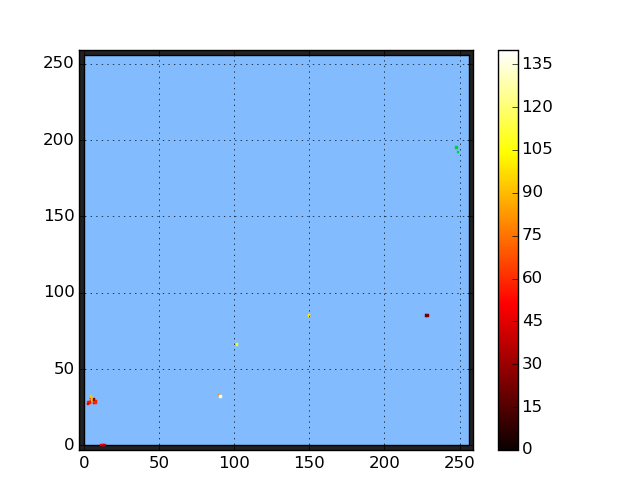
\includegraphics[width=0.7\textwidth]{assets/images/frame.png}
  \caption[The example output from the CERN@school job.]
  {\label{fig:localrunningframe}The example output from the CERN@school job.}
\end{figure}
%

For reference, that's a beta particle in the bottom left corner, and
five gammas in the rest of the frame! You can also find the source code
on the
\href{http://github.com/CERNatschool/particle-rate-plotter}{CERN@school
GitHub page}.
